% DPCN Assignment 1 report
% Compile: latexmk -xelatex report.tex
\documentclass[11pt,a4paper]{article}

\usepackage{fontspec}
\usepackage{libertinus-otf}

\usepackage[a4paper,margin=22mm]{geometry}
\usepackage{setspace}
\setstretch{1.12}
\usepackage{parskip}
\usepackage{microtype}
\usepackage{xcolor}
\usepackage{titlesec}
\usepackage{graphicx}
\usepackage{booktabs}
\usepackage{enumitem}
\usepackage{caption}
\usepackage{float}

\setlist[itemize]{leftmargin=1.35em,itemsep=0.12em,topsep=0.35em,parsep=0pt,partopsep=0pt}
\usepackage{fancyhdr}
\usepackage[hidelinks]{hyperref}
\usepackage{xurl}

\definecolor{ink}{HTML}{1C1C1C}
\definecolor{muted}{HTML}{5A5A5A}
\definecolor{rulec}{HTML}{2C3E50}
\color{ink}

\graphicspath{{../outputs/figures/}}

\titleformat{\section}{\sffamily\bfseries\large\color{rulec}}{\thesection.}{0.6em}{}
\titlespacing*{\section}{0pt}{1.3em}{0.45em}

\pagestyle{fancy}
\fancyhf{}
\fancyhead[L]{\sffamily\small\color{muted} DPCN Assignment 1: Opinion Network Formation}
\fancyhead[R]{\sffamily\small\color{muted} 1885smashburgers}
\fancyfoot[C]{\sffamily\small\thepage}
\renewcommand{\headrulewidth}{0.3pt}
\renewcommand{\footrulewidth}{0pt}
\setlength{\headheight}{14pt}

\captionsetup{font=small,labelfont={bf,sf},skip=4pt}

\begin{document}

\noindent
{\sffamily\bfseries\LARGE Assignment 1: Opinion Network Formation}\\[0.35em]
{\sffamily\large DPCN \textperiodcentered\ IIIT Hyderabad}\\[0.15em]
{\sffamily\color{muted} September 2026}

\vspace{0.4em}
{\color{rulec}\hrule height 0.8pt}
\vspace{0.9em}

\section{Team Name}

1885smashburgers. The team members are Bhavya Ahuja, Hasini, and Eshaan Sharma.

\section{GitHub Link to Code}

The code, survey CSV, figures, and this report live at
\url{https://github.com/bhavyahuja/DPCN-assignment-1}. Run \texttt{python run\_pipeline.py} from the project root to rebuild the network, metrics, and plots.

\section{Dataset Documentation}

The class survey is \textbf{60 Likert items} split evenly across four themes: \textbf{Technology} (T01--T15), \textbf{Education} (E01--E15), \textbf{Ethics/Society} (S01--S15), and \textbf{Environment} (V01--V15). The CSV had 96 rows. Five of those rows were completely empty, so we dropped them. That left \textbf{91 people} we actually use as nodes.

We coded the scale as Strongly Disagree~$=$~1, Disagree~$=$~2, Neutral~$=$~3, Agree~$=$~4, Strongly Agree~$=$~5. Anything that is not on that scale---blank cells and the odd ``No Comments''---is treated as missing. After dropping the empty rows, 242 cells are still missing, about \textbf{4.4\%} of the remaining answers. Missingness is spread across all four blocks, so one theme is not systematically worse than the others. When we compare two people we only use items both of them answered.

A few things about how we read the instrument:
\begin{itemize}
  \item Almost every statement is worded in a \textbf{positive direction}: AI will help, universities should do X, climate needs action. So a high mean is not ``left vs right.'' It is just ``this person agreed with most of the survey.''
  \item People also tend to sit on the \textbf{Agree} side, which matters later when we pick a similarity measure.
  \item This is \textbf{not a social network}. Nobody was asked who they talk to. An edge in our graph only means two answer sheets look alike.
\end{itemize}

\section{Pipeline Followed}

Each remaining respondent is a \textbf{60-dimensional opinion vector}. We first tried raw \textbf{cosine} similarity on those vectors and it was useless: because almost everyone is around Agree, cosine between two people is high even if they disagree on the items that actually vary. \textbf{Pearson} correlation (cosine after mean-centering) fixes that. It compares the \emph{shape} of two profiles---which items someone is relatively more or less on board with---instead of the fact that both of them said Agree a lot.

If we kept every positive correlation as an edge we would get a near-complete graph. Density would be high, communities would be mush, and there would be nothing interesting to report. So we sparsify with $k$-nearest neighbours, $k=8$:
\begin{itemize}
  \item For each person we keep their eight closest peers.
  \item We add an undirected edge if the link exists in either direction (\textbf{union $k$NN}, not strict mutual $k$NN). The edge weight is the Pearson correlation.
  \item Isolates, if any, get attached to their single best match so Louvain is not flooded with one-person ``communities.''
\end{itemize}

We run the same construction four more times, once per theme, using only that theme's 15 items. The \textbf{overall graph} is what we analyse in most of the report. The four theme graphs are there to check whether the class splits more on Technology than on Environment, which is something we actually expected going in.

After the graph is built we compute density, average degree, weighted clustering, shortest-path length and diameter on the giant component, plus \textbf{degree}, \textbf{betweenness}, and \textbf{eigenvector} centrality. Communities come from \textbf{Louvain} with edge weights equal to similarity and resolution 1. Betweenness uses distance $1 - \text{similarity}$, so a strong agreement is a short hop, not a long one. Each community then gets a mean Likert score on T/E/S/V so we can say what the cluster is actually agreeing with, not just that a cluster exists.

The overall network has \textbf{91 nodes}, \textbf{357 edges}, density 0.087, and average degree 7.85. It is a single connected component.

\section{Analysis and Visualizations}

Table~\ref{tab:global} is the summary. Average shortest path in the giant component is \textbf{2.59} hops and the diameter is \textbf{6}, which is about what you want from a $k$NN graph this size: people are a few steps apart, not a hairball and not a chain. Weighted clustering is 0.168. Louvain finds \textbf{five communities}, sizes 11, 23, 15, 20, and 22, with modularity \textbf{0.369}. That is high enough to say the class is not one blob. Students who look similar tend to look similar as a group.

\begin{table}[H]
\centering
\caption{Global metrics of the overall opinion network.}
\label{tab:global}
\small
\begin{tabular}{@{}lccccccc@{}}
\toprule
Nodes & Edges & Density & Avg.\ deg. & Clustering & ASP & Diameter & Modularity \\
\midrule
91 & 357 & 0.087 & 7.85 & 0.168 & 2.59 & 6 & 0.369 \\
\bottomrule
\end{tabular}
\end{table}

Centrality is easier to read as three separate rankings:
\begin{itemize}
  \item \textbf{Eigenvector} picks people who sit next to other well-connected people. Top IDs: 114 (0.307), 104 (0.298), 81 (0.259), 61 (0.221), 110 (0.217). We read them as a consensus core of the main cluster, not as influencers.
  \item \textbf{Betweenness} flags people on short paths between communities. Top IDs: 104 (0.166), 114 (0.143), 95 (0.089), 90 (0.080), 77 (0.076).
  \item \textbf{Degree} (sum of incident Pearson weights) is headed by 114 and 104 as well.
\end{itemize}
104 and 114 show up on both eigenvector and betweenness, so they are both typical of a dense region \emph{and} sit on bridges.

\begin{figure}[H]
\centering
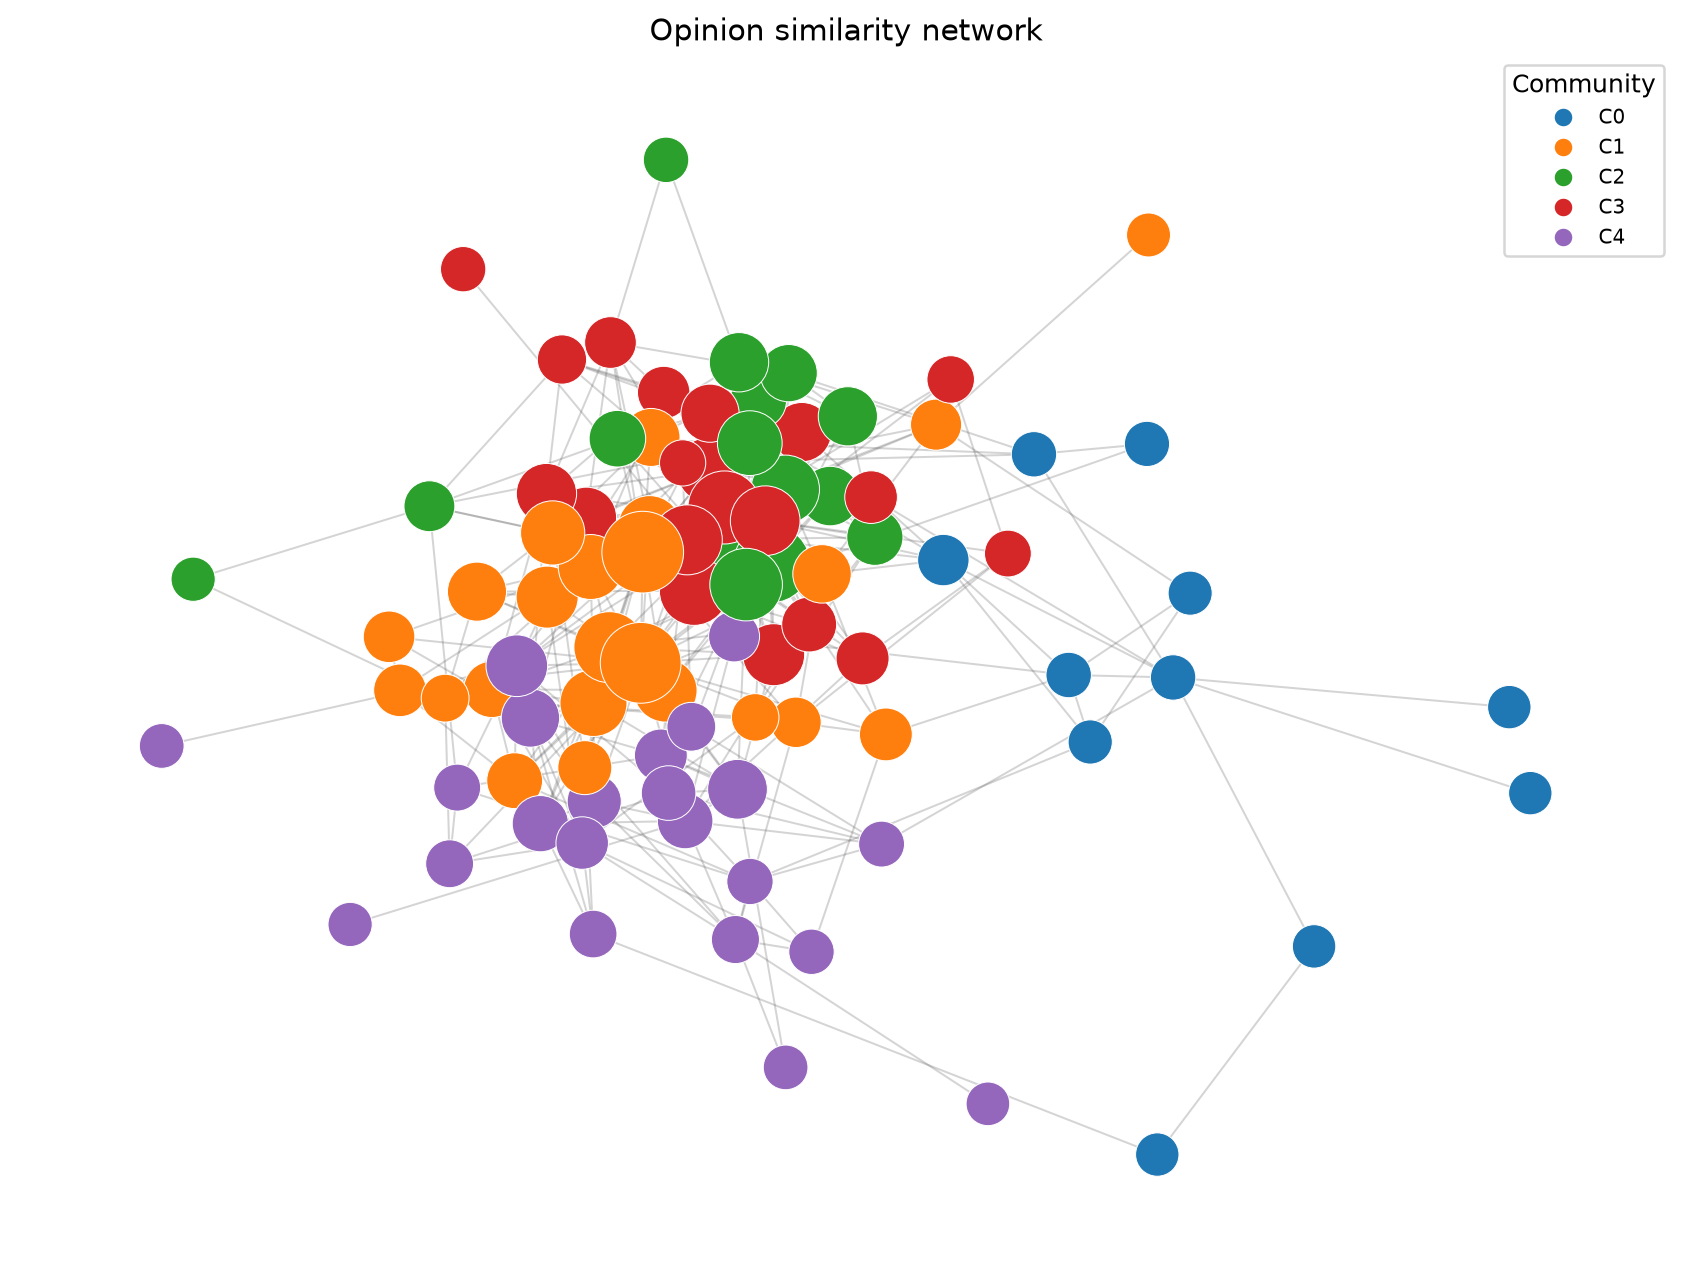
\includegraphics[width=0.92\textwidth]{network_overall.png}
\caption{Overall union-8NN opinion network. Node colour is Louvain community; node size is eigenvector centrality.}
\label{fig:net}
\end{figure}

Figure~\ref{fig:net} is the layout of that graph. Colour blobs are the five communities. Bigger nodes are the eigenvector core. You can see a large mixed middle and a few tighter pockets; nothing looks like two warring camps.

\begin{figure}[H]
\centering
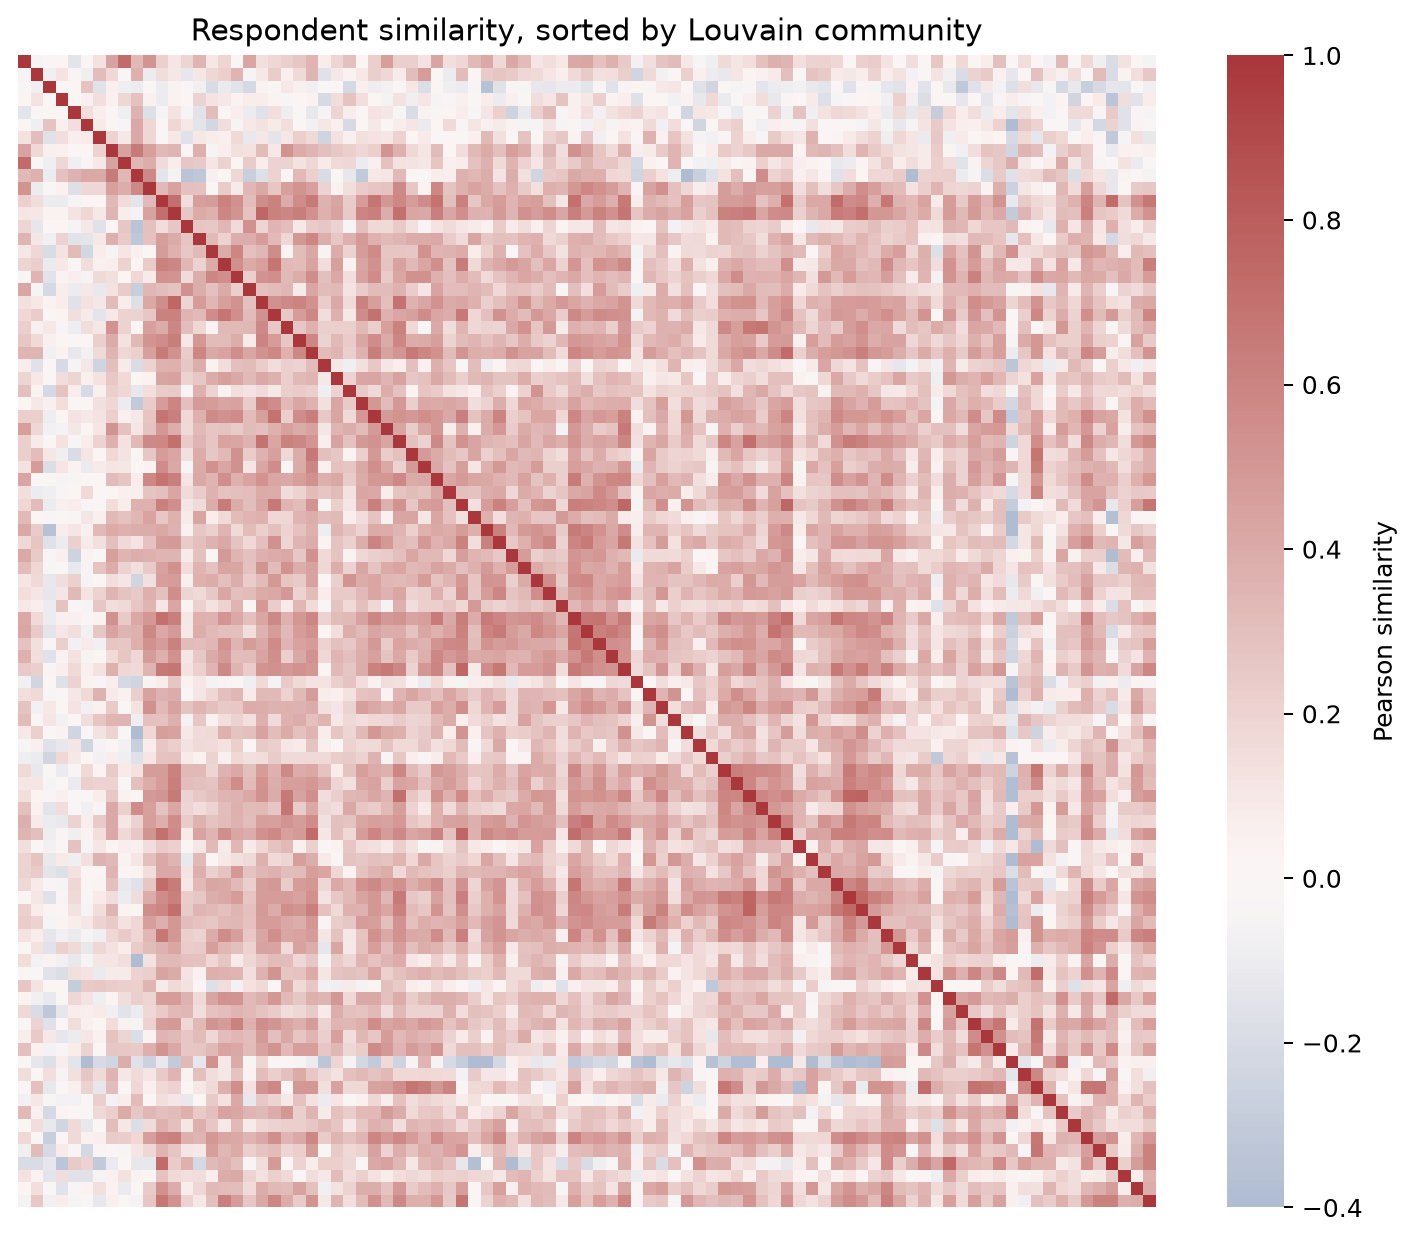
\includegraphics[width=0.78\textwidth]{heatmap.png}
\caption{Pearson similarity heatmap, respondents sorted by community. Warm blocks on the diagonal are within-community agreement.}
\label{fig:heat}
\end{figure}

The heatmap in Figure~\ref{fig:heat} is the same information without the layout algorithm. Sorting by community makes the diagonal blocks visible. Off-diagonal cells are cooler, which is the whole point of running Louvain: within-group correlation is higher than between-group correlation. The blocks are not jet black, though. People still agree with the other groups on a lot of items.

\begin{figure}[H]
\centering
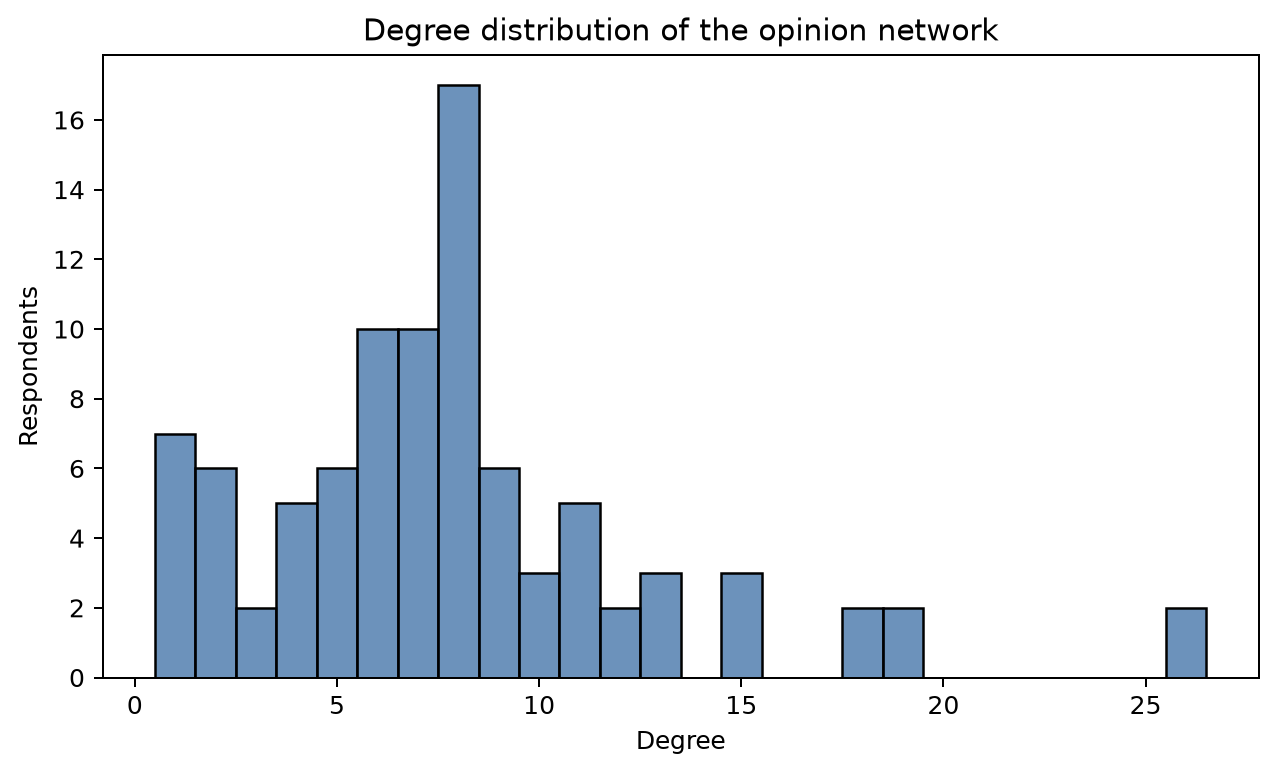
\includegraphics[width=0.82\textwidth]{degree_distribution.png}
\caption{Degree distribution. Most degrees sit near $k=8$; a few hubs go higher because many students list the same person as a neighbour.}
\label{fig:deg}
\end{figure}

Degree (Figure~\ref{fig:deg}) is peaked around 8, which is the $k$ we chose. A few nodes go past that because union $k$NN is not a hard cap: if many people name you as a neighbour, you pick up extra edges. That is a hub in \emph{this} construction, not a scale-free social graph. We would not over-read a power-law story into it.

\begin{figure}[H]
\centering
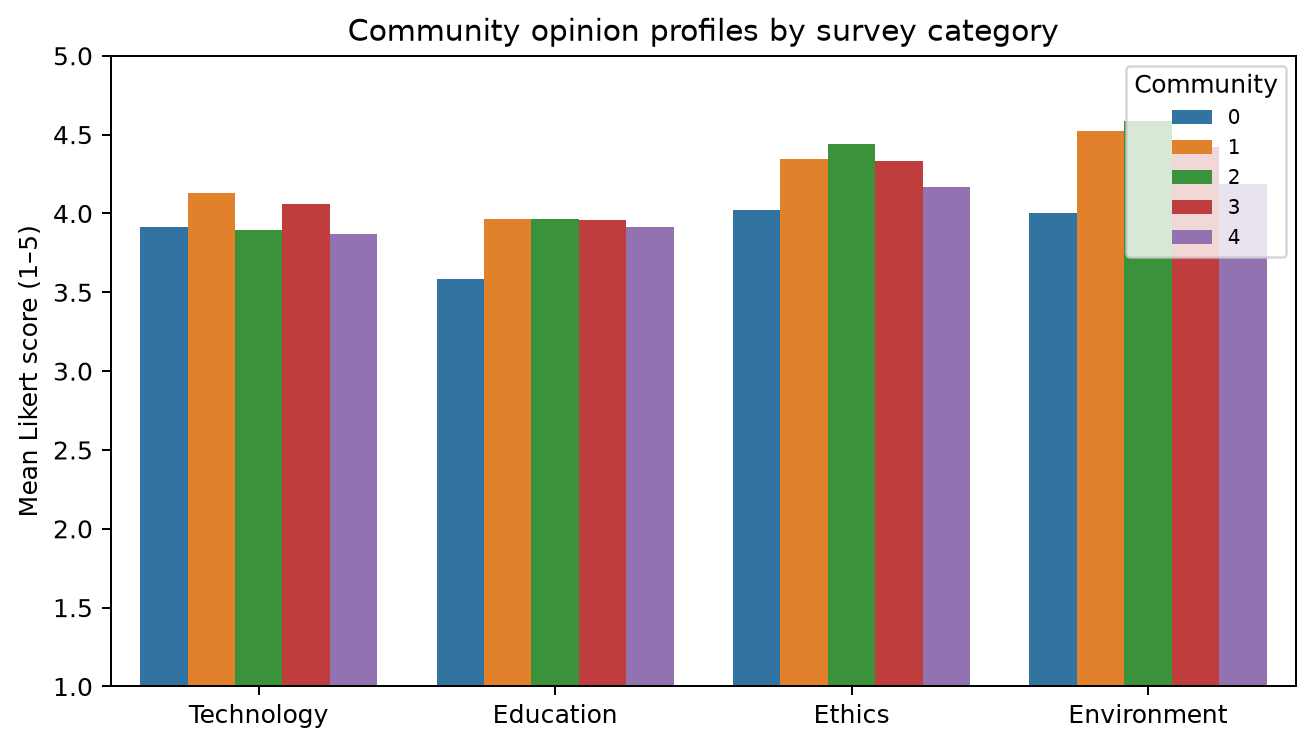
\includegraphics[width=0.88\textwidth]{community_profiles.png}
\caption{Mean Likert score (1--5) of each community on the four survey themes.}
\label{fig:prof}
\end{figure}

Figure~\ref{fig:prof} is the plot we actually care about for interpretation. Communities are not just colours on a graph; they have different average scores on Technology, Education, Ethics, and Environment. The range is still narrow---everyone is around Agree---but the gaps between communities are large enough to talk about.

\begin{figure}[H]
\centering
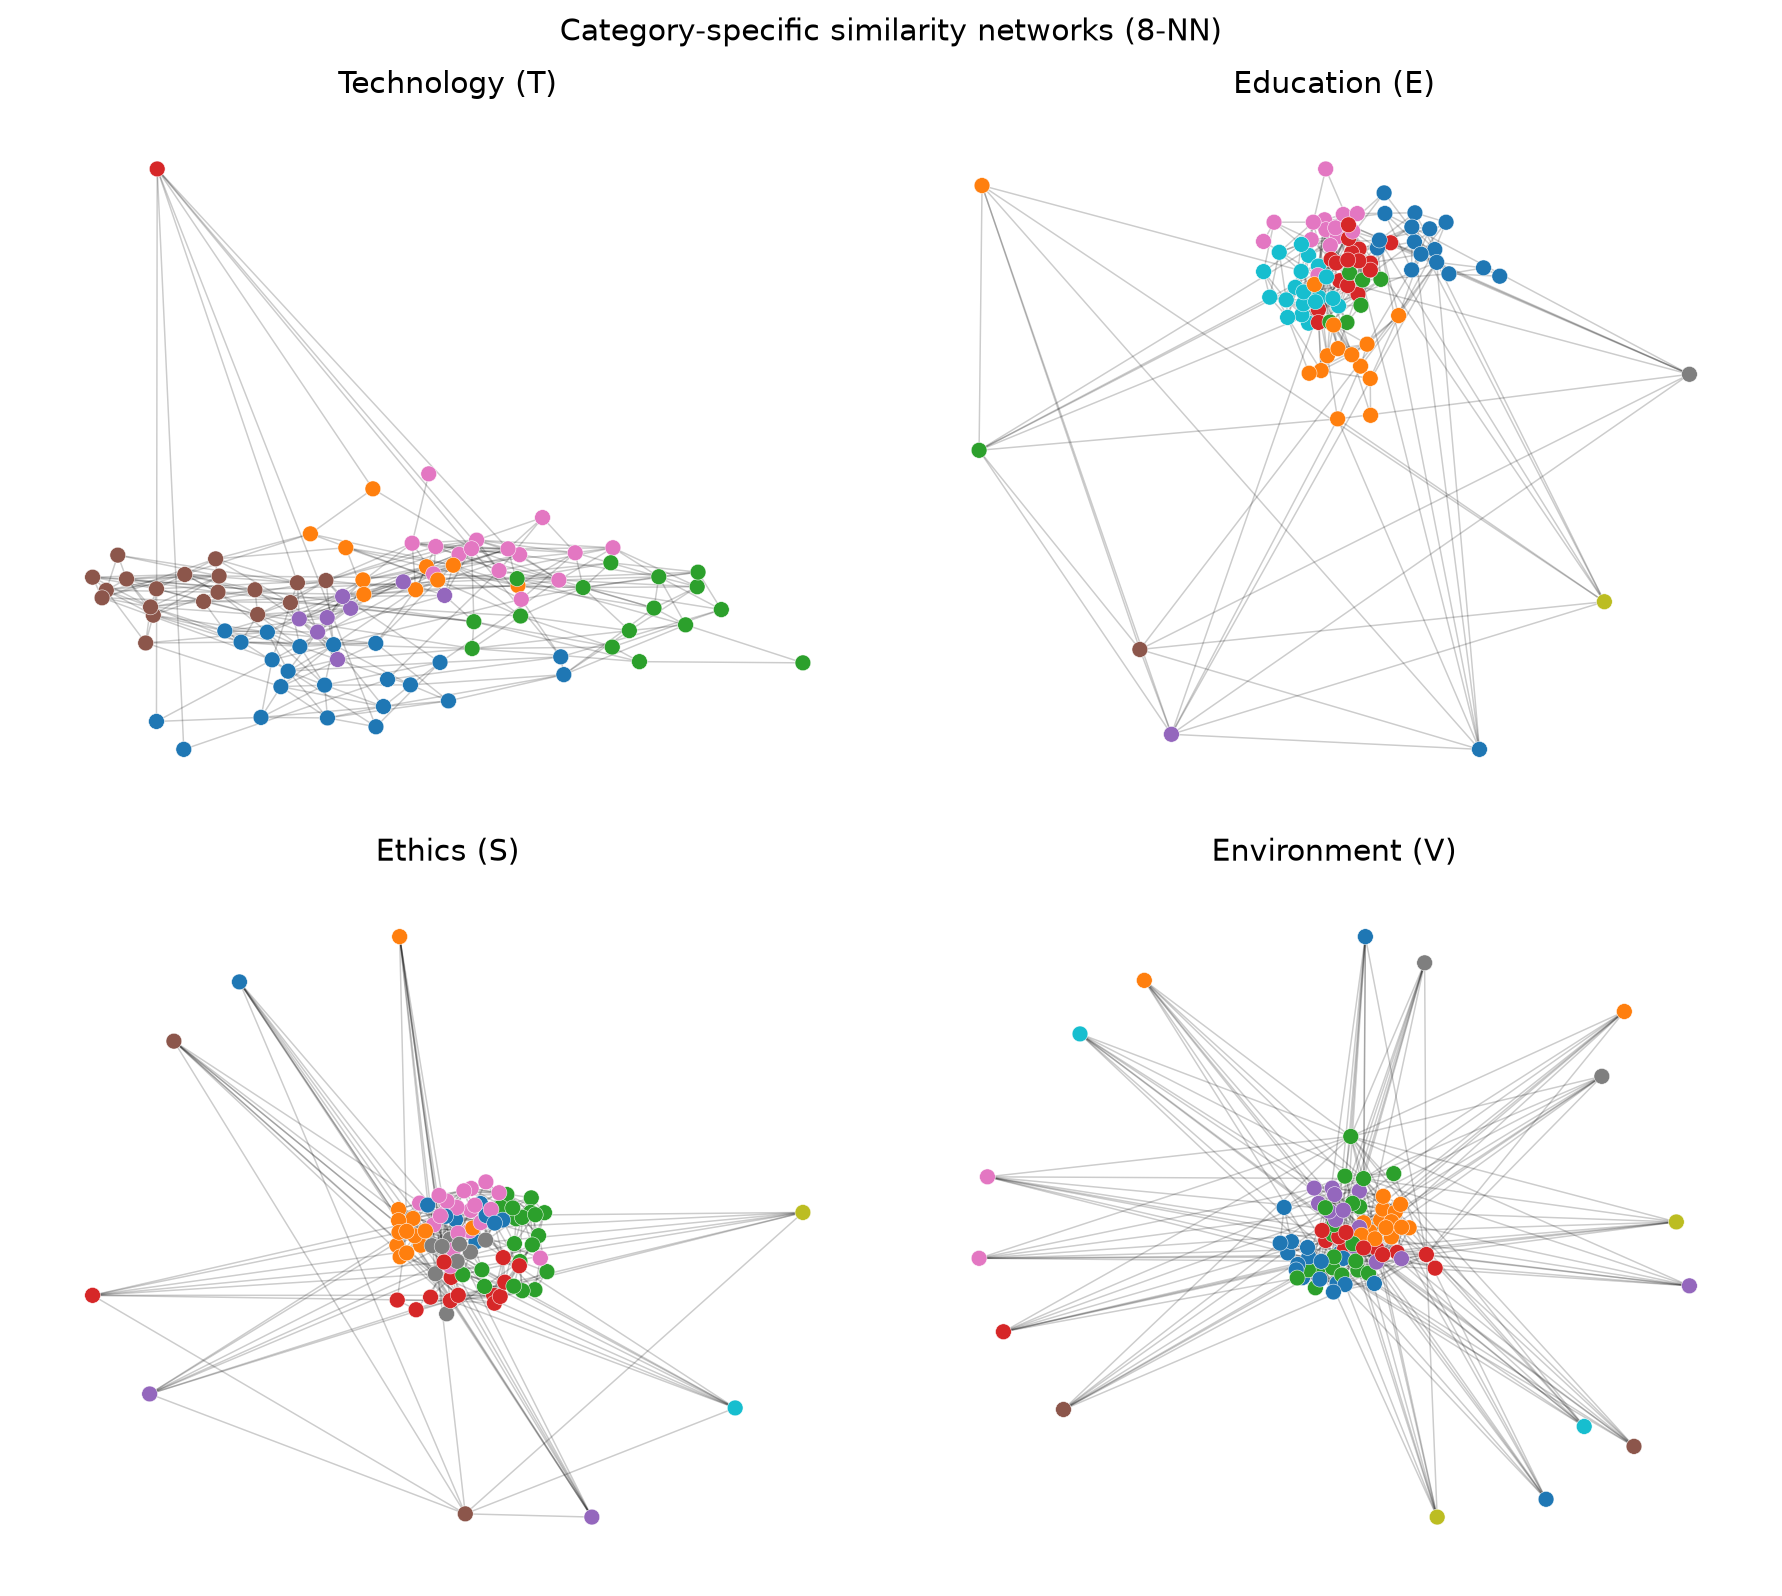
\includegraphics[width=0.90\textwidth]{category_networks.png}
\caption{Theme-specific 8NN networks built on the 15 Technology, Education, Ethics, and Environment items only.}
\label{fig:catnet}
\end{figure}

\begin{figure}[H]
\centering
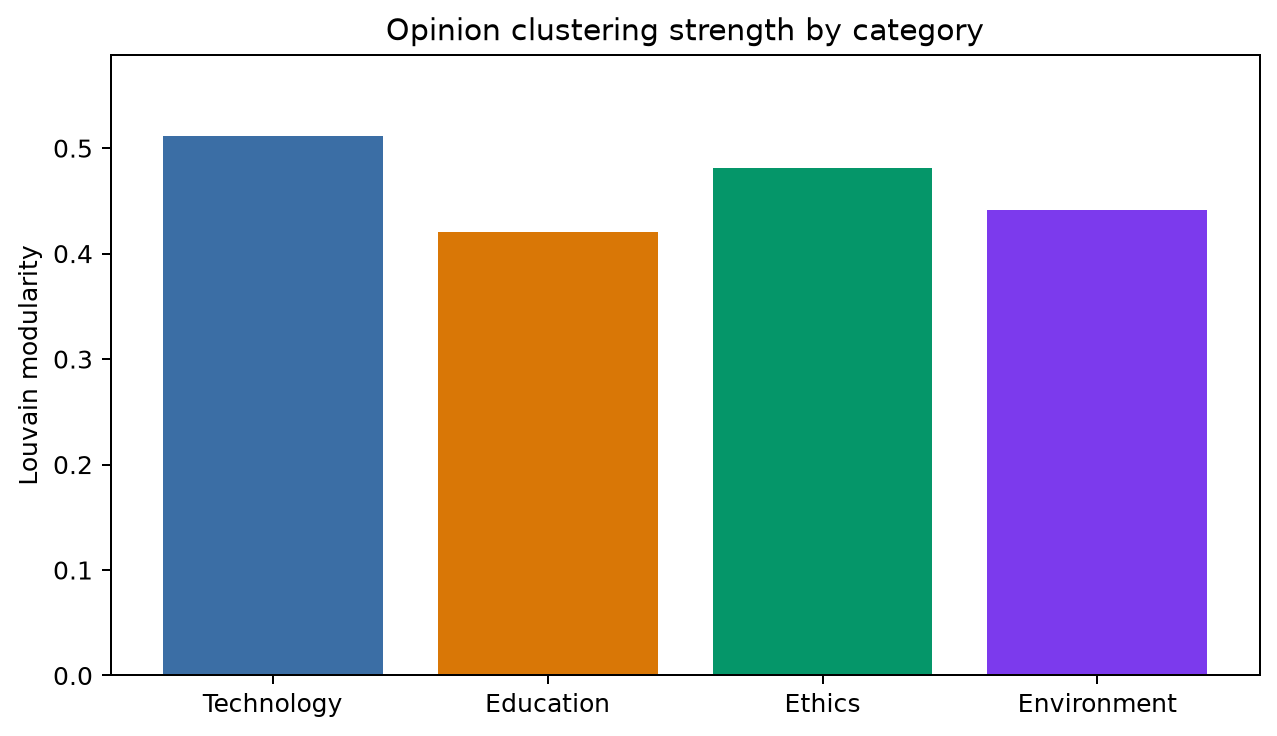
\includegraphics[width=0.78\textwidth]{category_modularity.png}
\caption{Louvain modularity of each theme-specific network.}
\label{fig:catmod}
\end{figure}

The four theme graphs (Figure~\ref{fig:catnet}) look similar at a glance, so we lean on the numbers in Figure~\ref{fig:catmod} and Table~\ref{tab:cat}.
\begin{itemize}
  \item \textbf{Technology} has the strongest clustering (modularity 0.511, 7 communities).
  \item \textbf{Ethics} is next (0.481). \textbf{Environment} is 0.442 and \textbf{Education} is 0.421.
  \item Environment also has the most Louvain groups (22), which we do \emph{not} read as ``the class is most divided on climate.'' Those items are almost uniformly endorsed, so small differences get turned into extra tiny partitions.
\end{itemize}
Higher modularity on Technology is the cleaner signal: AI, robots, regulation, and healthcare are where answer sheets actually disagree.

\begin{table}[H]
\centering
\caption{Theme-specific 8NN networks.}
\label{tab:cat}
\small
\begin{tabular}{@{}lccccc@{}}
\toprule
Theme & Edges & Density & Clustering & Modularity & Communities \\
\midrule
Technology & 354 & 0.086 & 0.211 & 0.511 & 7 \\
Education & 367 & 0.090 & 0.206 & 0.421 & 13 \\
Ethics & 393 & 0.096 & 0.172 & 0.481 & 16 \\
Environment & 432 & 0.105 & 0.144 & 0.442 & 22 \\
\bottomrule
\end{tabular}
\end{table}

\section{Results and Discussion}

The class does not have one opinion. Five Louvain groups and a modularity of 0.369 are enough to say that. At the same time, every community mean sits between about 3.88 and 4.24. Nobody is living on Strongly Disagree. The split we found is \textbf{enthusiastic vs.\ selective agreement}, not two opposite ideologies.

\begin{itemize}
  \item \textbf{Community 1} ($n=23$, overall 4.24) is the high-agreement group: Technology 4.13, Education 3.97, Ethics 4.34, Environment 4.52.
  \item \textbf{Community 2} ($n=15$, overall 4.22) looks similar on Ethics and Environment (4.44 and 4.59) but is cooler on Technology (3.90).
  \item \textbf{Community 3} ($n=20$, overall 4.19) sits in the middle of that high band.
  \item \textbf{Community 4} ($n=22$, overall 4.03) is a notch down on every theme.
  \item \textbf{Community 0} is the smallest and the most reserved ($n=11$, overall 3.88), and the dip is clearest on Education (3.59).
\end{itemize}
If we had to guess from the items, Community 0 is people who did not buy compulsory attendance, exam-as-truth, or similar education statements, not people who rejected the whole survey.

\textbf{Pearson} is doing the work here. If we had clustered on raw means we would have one ``agrees a lot'' pile and one ``agrees a bit less'' pile. The communities also differ in \emph{which} block they are relatively high on. Community 2 is the ``ethics and environment first, AI second'' shape. Community 1 is high across the board, especially environment. Community 0 is the one that actually pulls Education down. That is a more useful picture of an engineering class than a left--right cartoon.

The theme comparison lines up with how the questions read. \textbf{Technology} items mix things people fight about (autonomous vehicles, AI in healthcare, government regulation) with things they mostly like (AI in science, data protection). \textbf{Environment} items are almost all ``we should take this seriously,'' so the class agrees and the graph is denser (432 edges vs.\ 354 on Technology) with weaker clustering. We went in expecting that, and the modularity numbers match.

Centrality should not be oversold:
\begin{itemize}
  \item High \textbf{eigenvector} just means ``your answers look like the answers of other well-connected people in this graph.'' It is a typical voice of a cluster, not a campus influencer.
  \item High \textbf{betweenness} means you sit between clusters in opinion space. If this were a discussion network those people would be the ones who can translate one group's worries to another.
\end{itemize}
We do not have discussion data, so we stop at structure.

A few caveats, because they actually change how far we would push this:
\begin{itemize}
  \item \textbf{Similarity is not interaction:} two people with the same answers may have never spoken.
  \item $k=8$ is a choice; a different $k$ would change density and maybe the community count, though the heatmap does not depend on $k$.
  \item Pearson ignores overall enthusiasm on purpose, which is what we wanted, but it also means a uniformly Strongly Agree person and a uniformly Agree person look closer than they feel.
  \item Missing cells are only 4.4\%, but they are not guaranteed random.
\end{itemize}
None of that undoes the main result: the cohort forms a clustered similarity network, the clusters are mild, and Technology fragments the class more cleanly than Environment does.

\section{Individual Contribution}

Work was split along the pipeline.

\paragraph{Bhavya Ahuja.} Dataset and graph construction: loading the CSV, Likert encoding, dropping empty rows, missing-value handling, Pearson similarity, union-8NN graphs (overall and per theme), repository setup, \texttt{run\_pipeline.py}, and the GitHub repo.

\paragraph{Hasini.} Network analysis: global metrics, degree / betweenness / eigenvector centrality, Louvain communities, community opinion profiles, and the per-theme modularity comparison.

\paragraph{Eshaan Sharma.} Visualizations, the written analysis and discussion, and typesetting this report.

All three of us reviewed the figures, the numbers in \texttt{outputs/metrics.json}, and the final PDF.

\section{Metric definitions}

\begin{itemize}
  \item \textbf{Density:} fraction of possible undirected pairs that are edges. \textbf{Average degree:} $2m/n$.
  \item \textbf{Clustering:} NetworkX's weighted average clustering coefficient. \textbf{ASP} and \textbf{diameter} use hop distance on the giant component.
  \item \textbf{Weighted degree:} sum of incident Pearson weights. \textbf{Betweenness:} path length $1 - \text{similarity}$. \textbf{Eigenvector:} nodes similar to other high-scoring nodes.
  \item \textbf{Louvain modularity:} weight inside communities vs.\ a random graph with the same degree sequence.
  \item \textbf{Community profiles:} mean Likert scores, first averaged over items in a theme, then over members of the community.
\end{itemize}

To reproduce: create a virtualenv, \texttt{pip install -r requirements.txt}, run \texttt{python run\_pipeline.py}. Figures land in \texttt{outputs/figures/}. The report is \texttt{report/report.tex}; compile with \texttt{latexmk -xelatex report.tex} from the \texttt{report/} directory. Layout and Louvain seeds are fixed at 42.

\end{document}
